\chapter{Design\label{chap:design}}

\section{Secure Proxy}
In order to enable FlyTrap to make decisions on whether the requests for publishing or subscribing should be accepted or denied, a secure proxy needs to be established between the clients and the MQTT Broker. As the communication between the broker and the consumers happens on Transport Control Layer, it is possible to insert a middleman who would be capable of inspecting the packets flowing through, dissecting it for relevant information and finally make a decision about their future journey - all without the client ever knowing that someone has intercepted the connection. 
\begin{figure}[h]
    \centering
    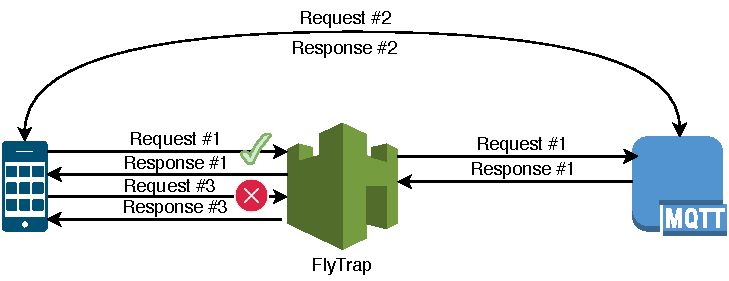
\includegraphics[width=0.8\textwidth]{tls}
    \caption{FlyTrap acting as a proxy}
    \label{fig:tls}
\end{figure}

Figure \ref{fig:tls} demonstrates all 3 possibilities when client attempts connection to a broker. In the Request \#1, FlyTrap will dissect the packet and confirm that the phone indeed can be allowed to access specific topic and then start bidirectional proxy with the broker, passing the TCP packets between two. Request \#2 shows that the same packet can be used for vanilla MQTT Broker without FlyTrap, thus decoupling the client and secure proxy, as the former can be used without the need to change the latter. Finally, for the third request, it is found that the client cannot access the requested resource and will be presented with CONACK response, with access denied flag set, terminating the connection.

Although this solution enough will not be sufficient, as quickly as FlyTrap can tap into the connection, the same can be assumed for potential malicious actors, which could be listening on the flowing through packets. The solution will support an extension to standard TCP - Transport Layer Security, or TLS for short, responsible for encrypting the TCP packets, significantly reducing the threat of man-in-the-middle attacks.

TLS sessions can be summarized in the following steps:
\begin{enumerate}
\item Initiate standard TCP session
\item ClientHello with client's cypher capabilities 
\item ServerHello and exchange of the cypher suite, along with server's certificate
\item Key exchange and change of cypher spec
\item Encrypted session starts
\end{enumerate}

It's important to point out, that due to step 3 requiring server's certificate, FlyTrap will need to either obtain a copy of broker's certificates or generate a new pair, ensuring that the connecting clients will trust it.


